\documentclass{article}

\usepackage[main=english,vietnamese]{babel}
\usepackage[T1]{fontenc}
\usepackage[utf8]{inputenc}
\usepackage[sexy]{evan}
\usepackage{matchsticks}
\usepackage{wrapfig}
\usepackage{listings}

\begin{otherlanguage*}{vietnamese}

\title{Một số bài đề xuất cho Pi 01, 2025}
\end{otherlanguage*}

\author{Nghia Doan}
\date{\today}

\begin{document}

\begin{otherlanguage*}{vietnamese}

\maketitle

\section{Đề bài}

\begin{problem*}[\textbf{1 (Mức B)}]
    \label{problem:pi-2025-1-p1}
    Tìm tất cả các cặp số nguyên $(x, y)$ sao cho:
    \[
        \frac{x^2 - 2025}{2x - 1} + \frac{y^2 - 2025}{2y - 1} = x + y.
    \]
\end{problem*}

\bigbreak

\begin{problem*}[{\textbf{2 (Mức B)}}]
    \label{problem:pi-2025-1-p2}
    Tìm tất cả các số nguyên dương $n$ có $k$ ($k \ge 3$) ước số: 
    \[ 
        1 = d_1 < d_2 < \ldots < d_k = n,
    \]
    sao cho $d_i$ chia hết $d_{i+2}$ với mọi $i=1,2, \ldots, k-2.$
\end{problem*}

\bigbreak

\begin{problem*}[{\textbf{3 (Mức A)}}]
    \label{problem:pi-2025-1-p3}
    $p$ và $q$ là hai số nguyên tố lẻ khác nhau. Chứng minh rằng nếu số nghiệm nguyên $(x,y)$ ($x \in \ZZ,\ y \in \ZZ$) của hệ bất phương trình sau:
    \[
        -\frac{q}{2} < py - qx < \frac{p}{2},\ 0 < x < \frac{p}{2},\ 0 < y < \frac{q}{2}
    \]
    là một số lẻ thì $p$ and $q$ là các số nguyên tố dạng $4k+3.$
\end{problem*}

\bigbreak

\begin{problem*}[{\textbf{4 (Mức A)}}]
    \label{problem:pi-2025-1-p3}
    Với mỗi số nguyên không âm $m,$ ký hiệu $f(m)$ là số chữ số 1 trong biểu diễn nhị phân của $m.$ $n$ là một số nguyên dương cho trước.
    Chứng minh rằng số
    \[
        \sum_{m=0}^{2^n - 1} \left( (-1)^{f(m)} \cdot 2^m \right)
    \]
    có ít nhất $n!$ ước số dương.
\end{problem*}

\newpage 

\section{Lời giải}

\begin{problem*}[\nameref{problem:pi-2025-1-p1}]
    Tìm tất cả các cặp số nguyên $(x, y)$ sao cho:
    \[
        \frac{x^2 - 2025}{2x - 1} + \frac{y^2 - 2025}{2y - 1} = x + y.
    \]
\end{problem*}

\begin{soln}
    Để ý rằng do $x$ và $y$ là hai số nguyên nên $2x-1 \ne 0$ và $2y-1 \ne 0.$
    Ngoài ra, $2025 = 45^2,$ do vậy để đơn giản hoá các biểu thức, đặt $k^2 = 2025,$
    ta có phương trình tương đương:
    \[
        \begin{array}{rclcl}
            & &(x^2 - k^2)(2y-1)+ (y^2 - k^2)(2x - 1) &=& (4xy-2x-2y+1)(x+y)\\
            \Leftrightarrow& &2xy(x+y) - (x^2+y^2) - 2k^2(x+y) + 2k^2 &=& 4xy(x+y) - 2(x+y)^2 + (x+y)\\
            \Leftrightarrow& &-2xy(x+y-1) + (x^2+2xy+y^2) - (2k^2+1)(x+y) + 2k^2 &=& 0\\
            \Leftrightarrow& &-2xy(x+y-1) + (x+y)^2 - (2k^2+1)(x+y) + 2k^2 &=& 0\\
            \Leftrightarrow& &-2xy(x+y-1) + (x+y-1)(x+y-2k^2) &=& 0\\
            \Leftrightarrow& &(x+y-1)(-2xy+x+y-2k^2) &=& 0\\
        \end{array}
    \]

    Ta xét hai trường hợp.

    \textit{Trường hợp 1:} $x+y-1=0,$ nên $y=1-x.$ Ta có nghiệm $(x,y) = (k, 1-k),$ với $k$ là số nguyên bất kỳ.
    
    \textit{Trường hợp 2:} $-2xy+x+y-2k^2=0.$ Phân tích ra thừa số, ta có:
    \[
        -2xy+x+y-2k^2=0 \Leftrightarrow 1 - 4k^2 = 1 - 2x - 2y + 4xy \Leftrightarrow (2x-1)(2y-1)=1-4k^2.
    \]
    
    Vì $k^2 = 2025,$ nên $1-4k^2 = -8099 = -7 \cdot 13 \cdot 89.$ Do đó $-8099$ có 16 cách phân thành tích hai số,
    nhưng vì ta có thể hoá đổi $x$ và $y$, do đó có 8 cách như sau:
    \[
        \begin{array}{rcccl}
            (2x-1)(2y-1) &=& 8099 \cdot (-1) &\Rightarrow& x = 4050,\ y = 0\\
            (2x-1)(2y-1) &=& 1157 \cdot (-7) &\Rightarrow& x = 579,\ y = -3\\
            (2x-1)(2y-1) &=& 623 \cdot (-13) &\Rightarrow& x = 312,\ y = -6\\
            (2x-1)(2y-1) &=& 91 \cdot (-89) &\Rightarrow& x = 46,\ y = -44\\
            (2x-1)(2y-1) &=& 89 \cdot (-91) &\Rightarrow& x = 45,\ y = -45\\
            (2x-1)(2y-1) &=& 13 \cdot (-623) &\Rightarrow& x = 7,\ y = -311\\
            (2x-1)(2y-1) &=& 7 \cdot (-1157) &\Rightarrow& x = 4,\ y = -578\\
            (2x-1)(2y-1) &=& 1 \cdot (-8099) &\Rightarrow& x = 1,\ y = -4049\\
        \end{array}
    \]

    Thực hiện hoán đổi các giá trị nhận được cho $x$ và $y$ cho trường hợp 2 và tổng hợp với các nghiệm của trường hợp 1,
    có thể kết luận các nghiệm của phương trình đã cho là $(k, 1-k),$ với mọi $k$ nguyên, $(4050, 0),$ $(579, -3),$ $(312, -6),$
    $(46, -44),$ $(45, -45),$ $(7, -311),$ $(4, -578),$ $(1, -4049),$ $(0, 4050),$ $(-3, 579),$ $(-6, 312),$
    $(-44, 46),$ $(-45, 45),$ $(-311, 7),$ $(-578, 4),$ và $(-4049, 1).$
\end{soln}

\begin{remark*}
    Xuất xứ của bài toán này là một bài toán luyện đội tuyển IMO của Canada. Bài gốc như sau.

    \bigbreak
    Tìm tất cả các cặp số nguyên $(x, y)$ sao cho:
    \[
        \frac{x^2 - 4}{2x - 1} + \frac{y^2 - 4}{2y - 1} = x + y.
    \]
\end{remark*}

\newpage

\begin{problem*}[\nameref{problem:pi-2025-1-p2}]
    Tìm tất cả các số nguyên dương $n$ có $k$ ($k \ge 3$) ước số $1 = d_1 < d_2 < \ldots < d_k = n,$
    sao cho $d_i$ chia hết $d_{i+2}$ với mọi $i=1,2, \ldots, k-2.$
\end{problem*}

\begin{soln}
    Dễ thấy do $n>1$ nên $n$ có ít nhất một ước số nguyên tố. Ta xét ba trường hợp dựa trên số lượng ước số nguyên tố của $n$.

    \textit{Trường hợp 1:} $n$ chỉ có một ước số nguyên tố.
    Dễ thấy rằng các số nguyên tố không thoả mãn điều kiện đề bài/ nhưng các luỹ thừa bậc hai trở lên của các số nguyên tố đều thoả mãn.

    \textit{Trường hợp 2:} $n$ chỉ có hai ước số nguyên tố khác nhau $p<q,$ $n=p^k q^{\ell},$ với $k$ và $\ell$ là hai số nguyên dương.

    \textit{Trường hợp 2a:} Nếu $k=1.$ Các ước số của $n$ có thể liệt kê theo thứ tự tăng dần như sau:
    \[
        1 = 1 < p < q < pq < \ldots < q^{i-1} < pq^{i-1} < q^{i} < \ldots < q^{\ell} < pq^{\ell} = n.
    \]

    Dễ thấy rằng mọi căp ước số $(d_i, d_{i+2})$ của $n$ chỉ có thể có một trong hai dạng $(q^{i}, q^{i+1})$ ($1 \le i \le \ell-1$), hoặc $(pq^{i}, pq^{i+1})$ ($1 \le i \le \ell-1$).
    Trong cả hai trường hợp $d_i \mid d_{i+2}.$

    \textit{Trường hợp 2b:} Nếu $k \ge 2.$ Khi này $p^2 \mid n.$ 
    
    Nếu $p^2 < q,$ khi đó tồn tại một số nguyên dương $2 \le i \le k $ sao cho $p^i < q,$ và các ước số của $n$ bé hơn hoặc bằng $q$ có thể liệt kê theo thứ tự tăng dần như sau:
    \[
        1 = 1 < p < p^2 < \ldots < p^i < q.
    \]

    Tuy vậy, điều này dẫn đến vì $p^{i-1} \mid q,$ với $i-1 \ge 1,$ vô lý. Do đó $q<p^2.$ 
    
    Nếu $\ell \ge 2,$ hay $q^2 \mid n.$ Khi này các ước số liên tiếp của $n$ theo thứ tự tăng dần từ $p$ đến $q^2$ như sau:
    \[
        1 = 1 < p < q < p^2 < pq < \ldots < q^2 \quad (1)
    \]

    Chú ý rằng giữa $pq$ và $q^2$ chỉ có thể có các luỹ thừa của $p$. Do đó có ít nhất hai ước số của $n$ đứng ngay trước $q^2$ trong chuỗi bất đẳng thức (1),
    đều nhỏ hơn và đều không chia hết $q^2.$
    
    Do đó, các ước số của $n = p^kq$ có thể liệt kê theo thứ tự tăng dần như sau:
    \[
        1 = 1 < p < q < p^2 < pq < p^2q < \ldots < p^{k-1}q < p^k < p^kq.
    \]

    Dễ thấy rằng mọi căp ước số $(d_i, d_{i+2})$ của $n$ có thể có hai dạng $(p^{i-1}q, p^{i}q)$ ($1 \le i \le k$), hoặc $(p^{i}, p^{i}q)$ ($1 \le i \le k$).
    Trong cả hai trường hợp $d_i \mid d_{i+2}.$ 
    
    \textit{Trường hợp 3:} $n$ có ít nhất ba ước số nguyên tố khác nhau $p<q<r.$
    Xét chuỗi bất đẳng thức:
    \[
        1 = 1 < p < \ldots < q < \ldots < r \quad (2)
    \]

    Dễ thấy rằng có ít nhất hai ước số của $n$ đứng ngay trước $r$ trong chuỗi bất đẳng thức (2) và cả hai đều không chia hết $r$.
    Do đó $n$ không thể là nghiệm.

    Ký hiệu $\mathcal{P}$ là tập hợp các số nguyên tố và $\ZZ^+$ là tập hợp các số nguyên dương, các nghiệm của bài toán là:
    \[
        \{ p^k \mid p \in \mathcal{P},\ k \in \ZZ^+,\ k \ge 2 \} \cup 
        \{ pq^{\ell} \mid p, q\ \in \mathcal{P},\ \ell \in \ZZ^+,\ p < q \} \cup
        \{ p^kq \mid p, q\ \in \mathcal{P},\ k \in \ZZ^+,\ p < q < p^2 \}
    \]
\end{soln}

\begin{remark*}
    Bài toán này dựa trên một số bài toán thường gặp trong các kỳ thi Olympic về quan hệ giữa các ước số.
\end{remark*}

\newpage

\begin{problem*}[\nameref{problem:pi-2025-1-p3}]
    $p$ và $q$ là hai số nguyên tố lẻ khác nhau. Chứng minh rằng nếu số nghiệm nguyên $(x,y)$ ($x \in \ZZ,\ y \in \ZZ$) của hệ bất phương trình sau:
    \[
        -\frac{q}{2} < py - qx < \frac{p}{2},\ 0 < x < \frac{p}{2},\ 0 < y < \frac{q}{2}
    \]
    là một số lẻ thì $p$ and $q$ là các số nguyên tố dạng $4k+3.$
\end{problem*}

\begin{proof}
    Để ý rằng:
    \[
        \begin{aligned}
            &-\frac{q}{2} < py - qx \Rightarrow py > qx - \frac{q}{2} \Rightarrow y > \frac{q}{p} x - \half \frac{q}{p}\\
            &py - qx < \frac{p}{2} \Rightarrow py < qx + \frac{p}{2} \Rightarrow y < \frac{q}{p} x + \half
        \end{aligned}
    \]

    Do vậy các điểm $P$ có toạ độ nguyên dương $(x,y)$ thoả mãn điều kiện đề bài là các điểm nằm bên trong \textit{hình chữ nhật}
    xác đinh bởi các cặp đường thẳng song song $(x = 0,\ x = \frac{p}{2}),$ và $(y=0,\ y=\frac{q}{2});$
    đồng thời nằm giữa \text{dải băng} xác đinh bởi hai đường thằng song song $y = \frac{q}{p} x + \half$ và $y = \frac{q}{p} x - \half \frac{q}{p}.$

    \textit{Ghi chú: Hai hình bên dưới minh hoạ cho hai trường hợp $(p,q) = (7,11)$ và $(p,q) = (7,13).$ 
    Các điểm màu cam là nghiệm của hệ bất phương trình.}
    \begin{center}
        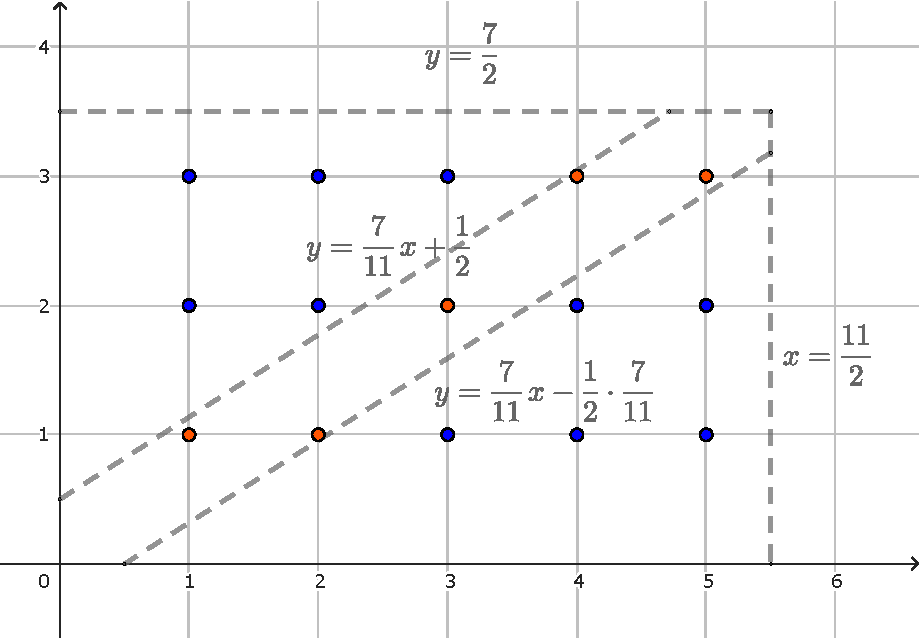
\includegraphics[width=7.5cm]{./svg/pdf/pi-2025-1-p3.pdf}
        \quad
        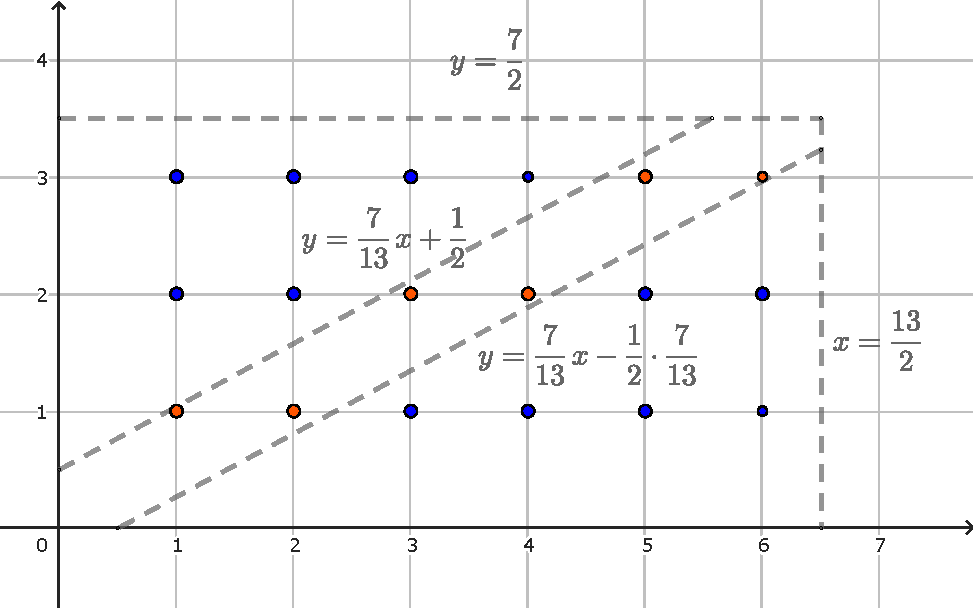
\includegraphics[width=8.5cm]{./svg/pdf/pi-2025-1-p3-2.pdf}
    \end{center}

    Theo điều kiện đề bài, không có nghiệm nào nào của hệ bất phương trình nằm trên chu vi của hình chữ nhật hoặc viền của dải băng.

    Chúng ta chứng minh hai tính chất sau.

    \begin{claim*}[Tính chất 1]
        Đường chéo qua gốc toạ độ của hình chữ nhật và hai đường viền của dải băng đều không chứa điểm có toạ độ nguyên dương $(x,y)$ nào.
    \end{claim*}
    \begin{subproof}
        Do đường chéo của hình chữ nhật đi qua hai điểm $(0,0)$ và $(\frac{p}{2}, \frac{q}{2})$ nên phương trình của đường là $py = qx.$
        Điểm $(x,y)$ có toạ độ nguyên dương nằm trên đường này nghĩa là tồn tại các số nguyên $0 < x < \frac{p}{2}, 0 < y < \frac{q}{2}$ sao cho $py = qx.$
        Điều này không thể xảy ra.

        Điểm $(x,y)$ có toạ độ nguyên dương nằm trên đường viền của dải băng tương đương sự tồn tại các số nguyên $0 < x < \frac{p}{2}, 0 < y < \frac{q}{2}$ 
        sao cho $py - qx = \frac{p}{2}$ hoặc $py - qx = -\frac{q}{2}$. Điều này dĩ nhiên cũng không xảy ra do $p$ và $q$ đều lẻ.
    \end{subproof}

\newpage

    \begin{claim*}[Tính chất 2]
        Đặt $T_1$ là hình tam giác xác định bởi các đường $y=0,$ $x=\frac{p}{2},$ và $y < \frac{q}{p} x + \half;$
        và $T_2$ là hình tam giác xác định bởi các đường $y=\frac{q}{2},$ $x=0,$ và $y > \frac{q}{p} x - \half \frac{q}{p}.$
        Số điểm có toạ độ nguyên trong $T_1$ và trong $T_2$ là như nhau.

        \textit{Ghi chú: Trong hai hình minh hoạ bên trên, các điểm trong hai tam giác $T_1$ và $T_2$ được tô màu xanh.}
    \end{claim*}
    \begin{subproof}
        Hàm $f: T_1 \rightarrow \RR^2$ được định nghĩa như sau:
        \[
            f((x,y)) = \left( \frac{p+1}{2} - x , \frac{q+1}{2} - y\right)
        \]

        Nếu $(x,y)$ là một điểm có toạ độ nguyên trong $T_1$ tương đương với: 
        \[
            0 < x < \frac{p}{2},\ 0 < y < \frac{q}{2},\ y < \frac{q}{p} x + \half.
        \]

        Do đó:
        \[
            \frac{1}{2} = \frac{p+1}{2} - \frac{p}{2} < \frac{p+1}{2} - x < \frac{p+1}{2} - 0 = \frac{p+1}{2} \Rightarrow 0 < \frac{p+1}{2} - x < \frac{p}{2} \quad (1)
        \]

        Tương tự như vậy 
        \[
            0 < \frac{q+1}{2} - y < \frac{q}{2} \quad (2)
        \]
        
        Ngoài ra:
        \[
            \frac{q+1}{2} - y > \frac{q}{p} \left(\frac{p+1}{2} - x \right) - \half \frac{q}{p}
            \Leftrightarrow\ \frac{q}{2} + \half -y > \frac{q}{p}\cdot \frac{p}{2} - \frac{q}{p}x
            \Leftrightarrow\ \half - y > -\frac{q}{p}x \Leftrightarrow y < \frac{q}{p} x + \half \quad (3)
        \]

        Từ (1), (2), và (3), ta suy ra
        \[
            \left( \frac{p+1}{2} - x , \frac{q+1}{2} - y\right) \in T_2 \Rightarrow f: T_1 \rightarrow T_2
        \]
        
        Dễ thấy rằng $f$ là một song ánh. Do đó số điểm có toạ độ nguyên trong $T_1$ và trong $T_2$ là như nhau.
    \end{subproof}

    Số điểm $(x,y)$ có toạ độ nguyên dương nằm bên trong hình chữ nhật xác đinh bởi các cặp đường thẳng song song 
    $(x = 0,\ x = \frac{p}{2}),$ và $(y=0,\ y=\frac{q}{2}),$ là $\frac{p-1}{2} \times \frac{q-1}{2}.$ 
    Do đó số điểm nguyên thoả mãn hệ bất phương trình bằng $\frac{p-1}{2} \times \frac{q-1}{2} - 2t,$ với $t$ là số điểm nguyên nằm trong tam giác $T_1$ (hoặc $T_2.$)
    Số điểm này là lẻ chỉ khi $p$ and $q$ là các số nguyên tố dạng $4k+3.$
\end{proof}

\begin{remark*}
    Bài toán này dựa ý tưởng chứng minh Luật tuơng hỗ bậc hai (Quadratic reciprocity) của Ferdinand Gotthold Eisenstein.
\end{remark*}

\newpage

\begin{problem*}[\nameref{problem:pi-2025-1-p3}]
    Với mỗi số nguyên không âm $m,$ ký hiệu $f(m)$ là số chữ số 1 trong biểu diễn nhị phân của $m.$ $n$ là một số nguyên dương cho trước.
    Chứng minh rằng số
    \[
        \sum_{m=0}^{2^n - 1} \left( (-1)^{f(m)} \cdot 2^m \right)
    \]
    có ít nhất $n!$ ước số dương.
\end{problem*}

\begin{soln}
    Ta chứng minh tính chất đơn giản sau.
    \begin{claim*}
        Nếu $u, v$ là hai số nguyên không âm khác nhau, thì $\gcd\left(2^{2^u}+1, 2^{2^v}+1\right) = 1.$
    \end{claim*}
    \begin{subproof}
        Không mất tính tổng quát, giả sử rằng $u < v$. Giả sử rằng $\gcd\left(2^{2^u}+1, 2^{2^v}+1\right) > 1.$
        Khi đó tồn tại số nguyên tố lẻ $p,$ sao cho $p \mid 2^{2^u}+1,\ p \mid 2^{2^v}+1.$ 
        Bởi vì:
        \[
            2^{2^v} - 1 = \underbrace{(2^{2^0} + 1)(2^{2^1} + 1) \cdots (2^{2^{v-1}} + 1)}_{2^{2^u}+1\ \text{là một trong các thừa số này}} 
            \Rightarrow p \mid  2^{2^v} - 1 \Rightarrow p \mid (2^{2^v}+1) - (2^{2^v} - 1) = 2 \Rightarrow p = 2.
        \]

        Điều này vô lý vì $p$ lẻ. Do đó $\gcd\left(2^{2^u}+1, 2^{2^v}+1\right) = 1.$
    \end{subproof}

    Để ý rằng mọi số nguyên từ 0 đến $2^n-1$ (bao gồm cả 0 và $2^n-1$)
    đều có một cách biểu diễn duy nhất bằng tổng của một số phần tử của tập hợp $\{2^0, 2^1, \ldots, 2^{n-1}\}.$
    Từ định nghĩa của $f(m),$ tổng được nêu trong để bài chính là:
    \[
        (-1)^n \cdot (2^{2^0} - 1)(2^{2^1} - 1) \cdots (2^{2^{n-1}} - 1).
    \]

    Bên cạnh đó, với $k \in \{1, 2, \ldots, n-1\}$:
    \[
        2^{2^k}-1 = (2^{2^1}-1)(2^{2^1}+1)(2^{2^2}+1)\cdots (2^{2^{k-1}}+1) = (2^{2^0}+1)(2^{2^1}+1)\cdots (2^{2^{k-1}}+1).
    \]

    Do đó:
    \[
        (-1)^n \cdot (2^{2^0} - 1)(2^{2^1} - 1) \cdots (2^{2^{n-1}} - 1)
        = (-1)^n \cdot (2^{2^0} + 1)^{n-1} (2^{2^1} + 1)^{n-2} \cdots (2^{2^{n-3}} + 1)^2 (2^{2^{n-2}} + 1)\quad (1)
    \]

    Chọn $p_1,$ $p_2,$ $\ldots,$ và $p_{n-1}$ lần lượt là $n-1$ ước số nguyên tố của $2^{2^0} + 1,$ $2^{2^1} + 1$, $\ldots,$ và $2^{2^{n-2}} + 1.$
    Theo tính chất đã chứng minh, các số nguyên tố này khác nhau, do đó $d = p_1^{n-1} p_2^{n-2} \cdots p_{n-1}^1$ là ước số dương của vế phải của (1).
    Do đó mỗi ước số của $d$ đều là ước số của vế phải (1). Số ước số dương của $d$ là:
    \[
        ((n-1)+1)((n-2)+1)\cdots(1+1)= n!.
    \]

    Đây chính là điều phải chứng minh.
\end{soln}

\begin{remark*}
    Bài toán này là một bài thi vòng sơ tuyển trước kỳ thi Olympiad của Canada.
\end{remark*}

\end{otherlanguage*}

\end{document}